\documentclass[conference]{IEEEtran}
\IEEEoverridecommandlockouts
% The preceding line is only needed to identify funding in the first footnote. If that is unneeded, please comment it out.
\usepackage{cite}
\usepackage{amsmath,amssymb,amsfonts}
\usepackage{algorithmic}
\usepackage{graphicx}
\usepackage{textcomp}
\usepackage{xcolor}
\usepackage{float}
\usepackage{amsmath}
%\usepackage{subcaption}
%\usepackage{subfig}
\usepackage{subfigure}
\DeclareMathOperator*{\argmax}{arg\,max}
\DeclareMathOperator*{\argmin}{arg\,min}

\def\BibTeX{{\rm B\kern-.05em{\sc i\kern-.025em b}\kern-.08em
    T\kern-.1667em\lower.7ex\hbox{E}\kern-.125emX}}
\begin{document}

\title{Comparison of Anomaly Detection between Statistical Method and Undercomplete Autoencoder\\
%{\footnotesize \textsuperscript{*}Note: Sub-titles are not captured in Xplore and
%should not be used}
%\thanks{Identify applicable funding agency here. If none, delete this.}
}

\author{\IEEEauthorblockN{Muhammad Ayaz Hussain}
\IEEEauthorblockA{\textit{dept. name of organization (of Aff.)} \\
\textit{name of organization (of Aff.)}\\
Bochum, Germany \\
email address}
\and
\IEEEauthorblockN{Muhammad Saif ur Rahman}
\IEEEauthorblockA{\textit{dept. name of organization (of Aff.)} \\
\textit{name of organization (of Aff.)}\\
Bochum, Germany \\
email address}
\and
\IEEEauthorblockN{Ioannis Iossifidis}
\IEEEauthorblockA{\textit{dept. name of organization (of Aff.)} \\
\textit{name of organization (of Aff.)}\\
Bochum, Germany \\
email address}

\and
\IEEEauthorblockN{}
\IEEEauthorblockA{\textit{ } \\
	\textit{ }\\
	}

\and

\IEEEauthorblockN{Christian Klaus}
\IEEEauthorblockA{\textit{dept. name of organization (of Aff.)} \\
	\textit{name of organization (of Aff.)}\\
	Bochum, Germany \\
	email address}

}

\maketitle

\begin{abstract}
This paper is concerned about the use of unsupervised learning (semi-supervised) algorithms in power consumption data, as well as the comparison of the performance between statistical method and Undercomplete Autoencoder in classification. As power consumption varies over time, therefore the labeled data created by that, becomes obsolete over times. Therefore, supervised learning is not a viable method in the prediction of energy consumption.
%This document is a model and instructions for \LaTeX.

\end{abstract}

%\begin{IEEEkeywords}
%component, formatting, style, styling, insert
%\end{IEEEkeywords}

\section{Introduction}
In modern days, the amount of energy consumption is becoming a more serious issue as several companies and industries are addressing this issue in order to contain their expenses as unexpected variations can incur additional operational costs to their facilities. These fluctuations in electricity consumption can arise from various factors such as excessive use of heavy equipment like electric heaters in winters, room coolers during the summers etc. In order to detect such variations or anomalies, anomaly detector algorithm is designed and implemented on the provided data.
Presently, it is very difficult to predict the energy consumption anomalies precisely, since there are many factors influencing the energy usage, such as weather condition \cite{bb0},  occupancy \cite{bb1} and operation of appliances \cite{bb2,bb3}. 

\section{Related Works}

Previous studies in data-driven building energy consumption prediction have utilized several methods such as Engineering methods \cite{bb4}, statistical method \cite{bb5}, Artificial Neural Networks (ANN) \cite{bb6,bb7}, support vector machines (SVM) \cite{bb8}, fuzzy logic and grey model techniques \cite{bb9}, decision trees \cite{bb10} etc. 

Also there have been some studies which compared the effectiveness of different algorithms in energy consumption prediction by comparing the results of two or more algorithms on a similar dataset. For example, Li et al. \cite{bb8} compared SVM and Back Propagation Neural Network (BPNN); Borges et al. \cite{bb11} compared SVM and Autoregressive (AR) Model; Xuemei et al. \cite{bb12}  compared LS-SVM and BPNN; Liu and Chen \cite{bb13}  compared Support Vector Regression (SVR) and ANN; Penya et al. \cite{bb14}  compared AR Model, ANN,autoregressive integrated moving average (ARIMA), and Bayesian Network; Platon et al. \cite{bb15}  compared ANN and Case based Reasoning (CBR); Jain et al. \cite{bb16} compared SVM and MLR; (this paper linked from somewhere else) Hou et al. \cite{bb17}  compared ARIMA and ANN (need to download paper);  Fan et al. \cite{bb18}  compared MLR, ARIMA, SVM, RF, MLP, BT, MARS, and kNN; Chou and Bui \cite{bb19}  compared ANN, SVM, CART, CHAID, and GLR; Edwards et al. \cite{bb20}  compared MLR, FFNN, SVM, LS-SVM, HME-FFNN, and FCM-FFNN; Li et al. \cite{bb21,bb22} compared SVM, BPNN, Radial Basis Function Neural Network(RBFNN), and General Regression Neural Network (GRNN); Dagnely et al. \cite{bb23} [22] compared Ordinary Least Squared (OLS) Regression and SVR; Massana et al. \cite{bb24} compared MLR, MLP, and SVR; and Fernandez et al. \cite{bb25}  compared AR, polynomial model, ANN, and SVM.

A hybrid neural net ARIMA have been used by Chou et al.\cite{bb29} to detect anomalies in the power consumption in an office space. In another paper, Capozolli et al. \cite{bb30} used Classification and Regression Tree (CART), K-Mean clustering, Artificial neural networks and basic ensembling method (ANN BEM) and Outlier Detection methods such as Generalized Extreme Studentized Deviation (GESD) and Peak detection method on a building cluster.




As far as the use of autoencoder for classification is concerned, those have been used in previous works for classification tasks such as Fan et al.\cite{bb26} which used autoencoder based unsupervised anomaly detection method on a building energy data on a single facility which was in detail as several variables were considered.

Autoencoder is also been used for unsupervised classification of the traffic flow of data packet in Internet \cite{bb27}.
Whereas, Qi et al. \cite{bb28} used stacked autoencoders to diagnose and classify the faults in a rotating machinery.







\section{Methodology}

\subsection{\label{sec:level1}	Data Exploration and Feature Vector Construction}

In order to select meaningful features to be implement Machine Learning
or Statistical Modeling, it was necessary to analyze the given data throughly. After a comprehensive analysis, it was decided that the amount of energy
consumption depends upon multiple factors, which are the store itself as
all stores differs from one another as each having its particular size, different
number of energy consuming equipments and even have different geographical
location which affect the amount of energy consumption. Aside from that,
time of the day is another factor as during working hours energy consumption
is higher. There is also a reduction in power consumption
during the day even when the store is closed.
The data consisted of the energy readings from 227 stores with 238 sensor values (certain stores had multiple sensors) taken every 15 minute which spanned over a period of 11 months. The provided data was then throughly examined and it was subdivided into 2 main categories which were working days and non-working days as energy consumption showed different trends in both categories. Therefore, a Feature Vector was developed which consisted of respective month, hour of the day, store number, energy consumed, a tag for working day or non-working day.


\subsection{\label{sec:level2}	Statistical Method for Anomaly Detection}
In order to detect the outliers, a feature vector was developed, which consisted of the hour of the day, store number, energy consumed, a tag for working and non-working day and on that data a modified version of Tuckey's test was performed, which involves the calculation of median of training data which is referred to $\mathit{Q}$2 and then again median of values lesser and greater than that of $\mathit{Q}$2  is calculated. Median of values lower than $\mathit{Q}$2  is refereed as $\mathit{Q}$1  (lower quartile) and those having greater than $\mathit{Q}$2 is referred as $\mathit{Q}$3  (upper quartile) as shown in Figure 8. 

After determining $\mathit{Q}$1 and $\mathit{Q}$3, then Interquartile Range (IQR) is calculated by subtracting the value at $\mathit{Q}$3 by $\mathit{Q}$1.


After determining $\mathit{Q}$1 and $\mathit{Q}$3, then Interquartile Range (IQR) is calculated by subtracting the value at $\mathit{Q}$3 by $\mathit{Q}$1.

\begin{equation}
IQR = Q3 - Q1
\end{equation}

After calculating the IQR, we use it to calculate the Tuckey's Fences or Inner Fences by the following equation,

\begin{equation}
InnerFenceLowerLimit = Q1 - \alpha (IQR)
\end{equation}
\begin{equation}
InnerFenceUpperLimit = Q1 + \alpha (IQR)
\end{equation}

where,

$\mathit{\alpha}$ is the factor which varies the inner fence limits.

\begin{figure}[t]
	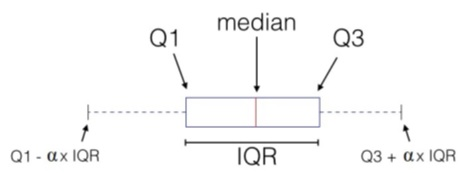
\includegraphics[width=\linewidth]{IQR.jpg}
	\caption{Depiction of quartiles as used in the detection and removal of
		Outliers.}
	\label{fig:boat0}
\end{figure}

Any value lying beyond inner fence limits (upper and lower) can be considered as an 	outlier, and therefore, it is removed. A sample result of designed outlier detection 	algorithm is shown in Figure \ref{fig:boat1} and \ref{fig:gull}.

As the dataset used in this project was highly varied and there were several energy values that stayed the same for the whole period of time. In order to calculate the quartiles and medians, there must be at least 4 unique values in a dataset, therefore for those dataset having less unique values, some product of their respective average was used to determine Inner and Outer Fences. 

\subsection{\label{sec:level3}	Autoencoders for Anomaly Detection}

An autoencoder always consists of two parts, the encoder and the decoder, which can be defined 	as transitions $\phi$ and $\psi$ such that:

\begin{equation}
\phi : \mathcal{X} \to \mathcal{F}
\end{equation}

\begin{equation}
\psi : \mathcal{F} \to \mathcal{X}
\end{equation}

\begin{equation}
\phi , \psi = 
\argmin_{\phi,\psi}\ \| X - (\phi \circ \psi)X  \|^2\\
\end{equation}

In a simple case, if there is one hidden layer, the encoder stage of an autoencoder takes the input $\mathbf{x}$ $\in$ $\mathbb{R}^d = \mathcal{X}$ and maps it to $\mathbf{z} \in \mathbb{R}^p =\mathcal{F}  $.
\begin{equation}
\boldmath{z} = \sigma(Wx+b)
\end{equation}

This image $\mathbf {z} $  is usually referred to as \textit{code}, \textit{latent variables} or \textit{latent representation}. Here, $\sigma$ is an element-wise activation function such as sigmoid function, hyperbolic tangent or a rectified linear unit. \boldmath{W} is weight matrix and \boldmath{b} is a bias vector. After that, the decoder stage of the autoencoder maps $\mathbf{z}$ to the reconstruction $\mathbf{x^{\prime}}$ of the same shape as $\mathbf{x}$.

\begin{equation}
\boldmath{x^{\prime}} = \sigma^{\prime}(W^{\prime}z+b^{\prime})
\end{equation}

where, $\sigma^{\prime}$, $W^{\prime}$ and $b^{\prime}$ for the decoder may differ in general from the corresponding $\sigma$, $W$ and $b$ for the encoder, depending on the design of the autoencoder.

Autoencoders are also trained to minimise reconstruction errors (such as squared errors):

\begin{equation}
\mathcal{L}(x,x^{\prime}) = \|x- \sigma^{\prime}(W^{\prime}(\sigma(Wx+b))+b^{\prime})\|^2
\end{equation}

where, $x$ is usually averaged over some input training set.

If the feature space $\mathcal{F}$  has lower dimensionality than the input space $\mathcal{X}$, then the feature vector $\phi(x)$ can be regarded as a compressed representation of the input $x$.  If the hidden layers are larger than the input layer, an autoencoder can potentially learn the identity function and become useless. However, experimental results have shown that autoencoders might still learn useful features in these cases.


In case of Undercomplete autoencoders, $\mathcal{F}$ has lower dimensionality than the input space $\mathcal{X}$, then the feature vector $\phi(x)$  can be regarded as a compressed representation of the input $x$.

In our project, the Autoencoder was trained in a semi-supervised fashion on the values of normal energy consumption data. Afterwards, the trained model was used and evaluated on a pre-trained dataset. 


\section{\label{sec:level1}	Experiments and Results}

Outlier detection algorithm was developed and it performed adequately in removing the outliers. Figure \ref{fig:OLX} shows the energy consumption data of each hour for all working days in January 2016, where as, Figure \ref{fig:OLX1} shows the
same data as in figure \ref{fig:OLX} after the outlier removal algorithm implemented
on it
\begin{figure*}[h]
	\centering
	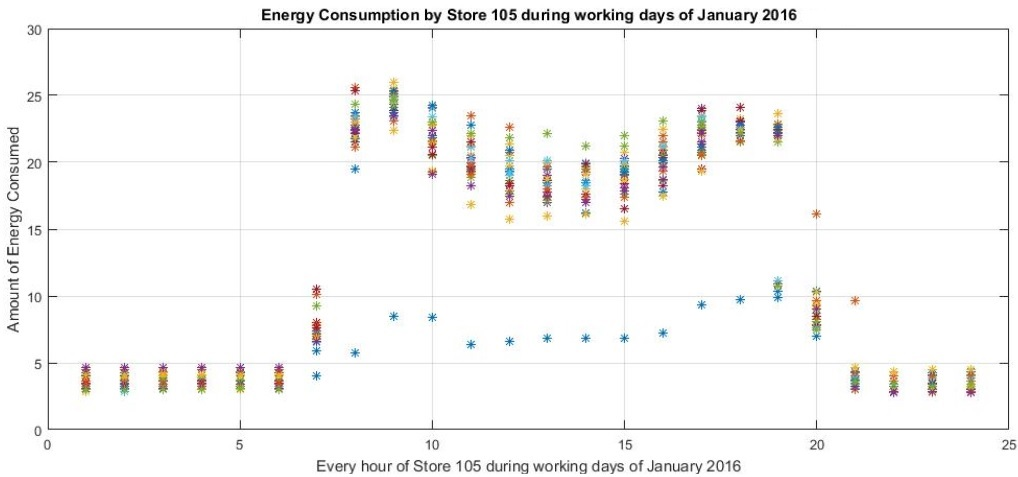
\includegraphics[width=13cm,height=6cm]{with_OL.jpg}
	\caption{Energy Consumption by Store 105 during working days of January
		2016 with outliers}
	\label{fig:OLX}
\end{figure*}
\begin{figure*}[h]
	\centering
	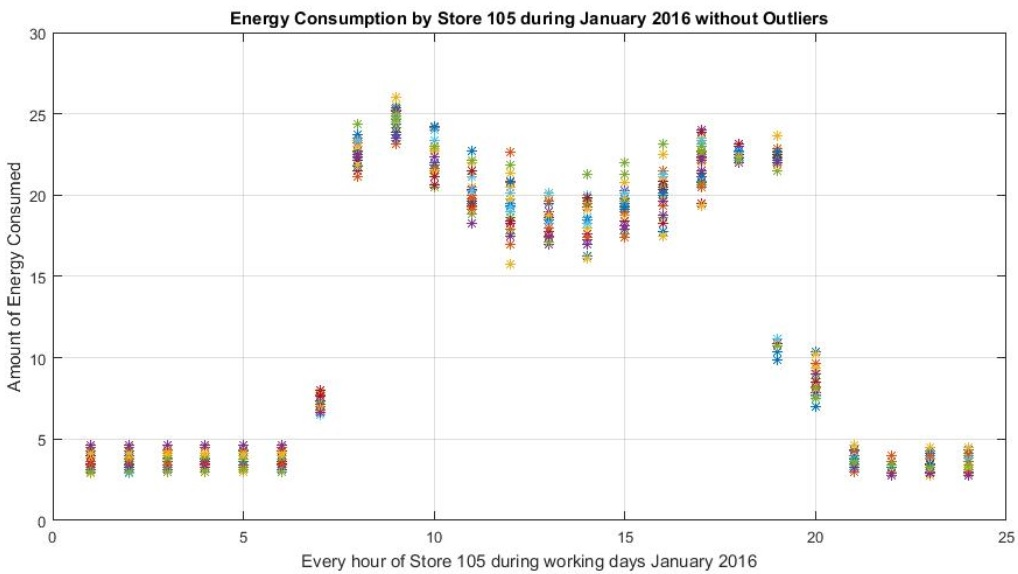
\includegraphics[width=13cm,height=6cm]{without_OL.jpg}
	\caption{Energy Consumption by Store 105 during working days of January
		2016 without outliers}
	\label{fig:OLX1}
\end{figure*}

\begin{figure}[h]
	\centering
	\subfigure[ROC curve of Anomaly Detection Algorithm.]
	{
		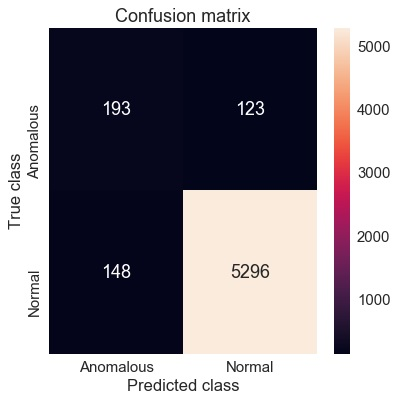
\includegraphics[width=3.0in]{conf_anomaly.jpg}
		%\caption{ROC curve of Anomaly Detection Algorithm.}
		\label{fig:boat1}
	}
	\\
	\subfigure[Confusion Matrix of Autoencoder.]
	{
		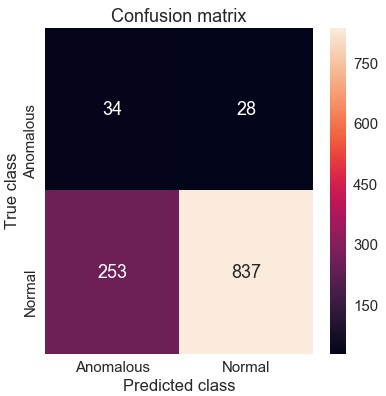
\includegraphics[width=3.0in]{Conf_autoencoder.jpg}
		\label{fig:boat2}
	}
	\caption{Confusion Matrices}
	\label{fig:conf}
\end{figure}

%\begin{figure}[]
%	%\centering
%	\begin{subfigure}{0.43\textwidth}
%		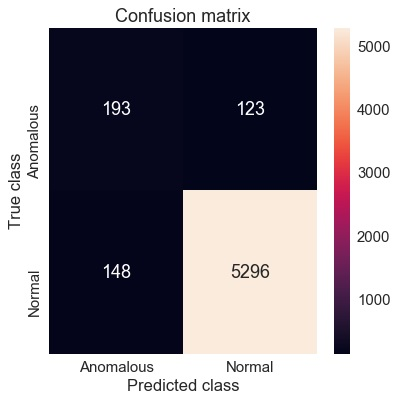
\includegraphics[width=\linewidth]{conf_anomaly.jpg}
%		\caption{Confusion Matrix of Anomaly Detection Algorithm}
%		\label{fig:boat1}
%	\end{subfigure}

%	\begin{subfigure}{0.43\textwidth}
%	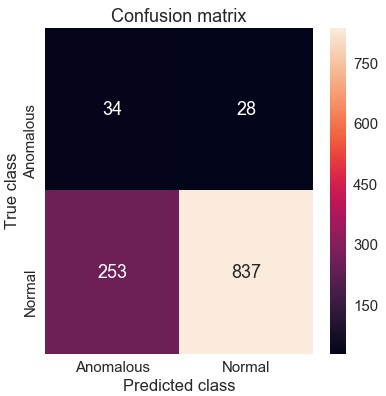
\includegraphics[width=\linewidth]{Conf_autoencoder.jpg}
%	\caption{Confusion Matrix of Autoencoder.}
%	\label{fig:boat2}
%\end{subfigure}
%\caption{Confusion Matrices}
%\label{fig:conf}
%\end{figure}



%\begin{figure}[h]
%	\centering
%	\begin{subfigure}{0.45\textwidth}
%		\includegraphics[width=\textwidth]{roc_anomaly.jpg}
%		\caption{ROC curve of Anomaly Detection Algorithm.}
%		\label{fig:gull}
%	\end{subfigure}
	~ %add desired spacing between images, e. g. ~, \quad, \qquad, \hfill etc. 
	%(or a blank line to force the subfigure onto a new line)
%	\begin{subfigure}{0.45\textwidth}
%		\includegraphics[width=\textwidth]{roc_autoencoder.jpg}
%		\caption{ROC curve of Autoencoder.}
%		\label{fig:tiger}
%	\end{subfigure}
%	\caption{ROC curves}
%	\label{fig:ROC}
	
%\end{figure}
\begin{figure}[H]
	\centering
	\subfigure[ROC curve of Anomaly Detection Algorithm.]
	{
		\includegraphics[width=3.5in]{roc_anomaly.jpg}
		
		\label{fig:gull}
	}
	\\
	\subfigure[ROC curve of Autoencoder.]
	{
		\includegraphics[width=3.5in]{roc_autoencoder.jpg}
		\label{fig:tiger}
	}
	\caption{ROC curves}
	\label{fig:ROC}
	
\end{figure}




In Fig \ref{fig:conf}, we are comparing the accuracy of prediction of both algorithms with manually classified energy data of two stores using confusion matrices. 


The same dataset which was used to make confusion matrices in Fig \ref{fig:conf} is used to plot Receiver Operating Characteristics curves in Fig \ref{fig:ROC}.




As we can see from the comparison of Fig \ref{fig:conf} and Fig \ref{fig:ROC}, we can interpret that the performance of Statistical method which is based on Tuckey's test performed remarkably better with around 95\% similarity with manual classification but the shortcoming of this method is that the dataset should be arranged in a proper manner as a single missing values in the dataset can make the classification ineffective. Whereas, classification using Autoencoder performed adequately with around 70-75\% correlation with manually classified data but it required pre-classified data containing no anomalies.  
 
 \section{Discussion/Outlook/Conclusion/Future Work}
 
 In this paper, the performance of a semi supervised Autoencoder and a statistical model for outlier detection was compared. The experiment resulted in the varying results from each algorithms as Autoencoder did not require data to be arranged precisely and were robust against mixed up dataset whereas, Statistical based outlier detection model performed more accurately in detecting outliers but it required careful arrangement of the data.
 
  
 In future, it is planned to use more variables in the feature vector of energy consumption data such size of the facility, number of energy consuming equipments, occupancy of the building, and other sensor data such as outside temperature and solar radiation. As more data is embedded in the feature vector, there will be more focus on using totally unsupervised learning using Autoencoder to discover and learn new pattern in the given dataset and do the classification more precisely. 
 
\begin{thebibliography}{00}
	
\bibitem{bb0} Liping Wang, Paul Mathew, and Xiufeng Pang. Uncertainties
in energy consumption introduced by building operations and
weather for a medium-size office building. \textit{Energy and Buildings},
53:152-158, 2012.
\bibitem{bb1} X. Feng, D. Yan, and T. Hong, "Simulation of occupancy in
buildings, energy and buildings," pp. 348-359, 2015. [Online].
	Available: http://www.sciencedirect.com/science/article/pii/
	S0378778806002404
\bibitem{bb2} H. Chenglei, L. Kangji, L. Guohai, and P. Lei, "Forecasting
building energy consumption based on hybrid pso-ann prediction model," in \textit{2015 34th Chinese Control Conference (CCC)},
July 2015, pp. 8243-8247.

\bibitem{bb3} M. Royapoor and T. Roskilly, "Building model calibration
using energy and environmental data," \textit{Energy and Buildings},
vol. 94, pp. 109 - 120, 2015. [Online]. Available: http://www.
	sciencedirect.com/science/article/pii/S0378778815001553
	
\bibitem{bb4}H. xiang Zhao and F. Magouls, "A review on the prediction
of building energy consumption," \textit{Renewable and Sustainable
Energy Reviews}, vol. 16, no. 6, pp. 3586 - 3592, 2012. [Online].
	Available: http://www.sciencedirect.com/science/article/pii/
	S1364032112001438
\bibitem{bb5}F. Lei and P. Hu, "A baseline model for office building energy
consumption in hot summer and cold winter region," in 2009
\textit{International Conference on Management and Service Science},
Sept 2009, pp. 1-4.

\bibitem{bb6}B. Bekta Ekici and U. Aksoy, "Prediction of building energy
consumption by using artificial neural networks," vol. 40, pp.
356-362, 05 2009.

\bibitem{bb7}A. Kusiak, M. Li, and Z. Zhang, "A data-driven approach for
steam load prediction in buildings," \textit{Applied Energy}, vol. 87,
no. 3, pp. 925 - 933, 2010. [Online]. Available: http://www.
	sciencedirect.com/science/article/pii/S0306261909003808
\bibitem{bb8}Q. Li, Q. Meng, J. Cai, H. Yoshino, and A. Mochida, "Applying
support vector machine to predict hourly cooling load in
the building," \textit{Applied Energy}, vol. 86, no. 10, pp. 2249 -
	2256, 2009. [Online]. Available: http://www.sciencedirect.com/
	science/article/pii/S0306261908003176
\bibitem{bb9}J. Guo, J. Wu, and R. Wang, "A new approach to energy
consumption prediction of domestic heat pump water heater
based on grey system theory," \textit{Energy and Buildings}, vol. 43,
no. 6, pp. 1273 - 1279, 2011. [Online]. Available: http://www.
	sciencedirect.com/science/article/pii/S0378778811000107
\bibitem{bb10}G. K. Tso and K. K. Yau, "Predicting electricity energy
consumption: A comparison of regression analysis, decision tree and neural networks," \textit{Energy}, vol. 32, no. 9, pp. 1761 -
	1768, 2007. [Online]. Available: http://www.sciencedirect.com/
	science/article/pii/S0360544206003288
	
\bibitem{bb11}C. E. Borges, Y. K. Penya, I. Fernndez, J. Prieto, and O. Bretos,
"Assessing tolerance-based robust short-term load forecasting in
buildings," \textit{Energies}, vol. 6, no. 4, pp. 2110-2129, 2013. [Online].
	Available: http://www.mdpi.com/1996-1073/6/4/2110
\bibitem{bb12} L. Xuemei, L. Jin-hu, D. Lixing, X. Gang, and L. Jibin, "Building
cooling load forecasting model based on ls-svm," in \textit{2009 AsiaPacific Conference on Information Processing}, vol. 1, July 2009,
pp. 55-58.
\bibitem{bb13}D. Liu and Q. Chen, "Prediction of building lighting energy consumption based on support vector regression," in \textit{2013 9th Asian
Control Conference (ASCC)}, June 2013, pp. 1-5.
\bibitem{bb14}Y. K. Penya, C. E. Borges, D. Agote, and I. Fernndez, "Shortterm load forecasting in air-conditioned non-residential buildings," in \textit{2011 IEEE International Symposium on Industrial
Electronics}, June 2011, pp. 1359-1364.
\bibitem{bb15} R. Platon, V. R. Dehkordi, and J. Martel, "Hourly prediction of
a building’s electricity consumption using case-based reasoning,
artificial neural networks and principal component analysis,"
\textit{Energy and Buildings}, vol. 92, pp. 10 - 18, 2015. [Online].
	Available: http://www.sciencedirect.com/science/article/pii/
	S0378778815000651
\bibitem{bb16} R. K. Jain, T. Damoulas, and C. E. Kontokosta, \textit{Towards
Data-Driven Energy Consumption Forecasting of Multi-Family
Residential Buildings: Feature Selection via The Lasso.}
[Online]. Available: https://ascelibrary.org/doi/abs/10.1061/
9780784413616.208

\bibitem{bb17} Z. Hou, Z. Lian, Y. Yao, and X. Yuan, "Cooling-load prediction
by the combination of rough set theory and an artificial neuralnetwork based on data-fusion technique," \textit{Applied Energy},
vol. 83, no. 9, pp. 1033 - 1046, 2006. [Online]. Available: http://
	www.sciencedirect.com/science/article/pii/S0306261905001315
\bibitem{bb18} C. Fan, F. Xiao, and S. Wang, "Development of prediction models for next-day building energy consumption and peak
power demand using data mining techniques," \textit{Applied Energy},
vol. 127, pp. 1 - 10, 2014. [Online]. Available: http://www.
	sciencedirect.com/science/article/pii/S0306261914003596
\bibitem{bb19} J.-S. Chou and D.-K. Bui, "Modeling heating and cooling loads
by artificial intelligence for energy-efficient building design,"
\textit{Energy and Buildings}, vol. 82, pp. 437 - 446, 2014. [Online].
	Available: http://www.sciencedirect.com/science/article/pii/
	S037877881400574X
\bibitem{bb20} R. E. Edwards, J. New, and L. E. Parker, "Predicting
future hourly residential electrical consumption: A machine
learning case study," \textit{Energy and Buildings}, vol. 49, pp. 591 -
	603, 2012. [Online]. Available: http://www.sciencedirect.com/
	science/article/pii/S0378778812001582
\bibitem{bb21}Q. Li, Q. Meng, J. Cai, H. Yoshino, and A. Mochida,
"Predicting hourly cooling load in the building: A comparison of
support vector machine and different artificial neural networks,"
\textit{Energy Conversion and Management}, vol. 50, no. 1, pp. 90
- 96, 2009. [Online]. Available: http://www.sciencedirect.com/
	science/article/pii/S0196890408003154
\bibitem{bb22} Q. Li, P. Ren, and Q. Meng, "Prediction model of annual energy consumption of residential buildings," in \textit{2010 International
Conference on Advances in Energy Engineering}, June 2010, pp.
223-226.
\bibitem{bb23}P. Dagnely, T. Ruette, T. Tourw, E. Tsiporkova, and C. Verhelst,
"Predicting hourly energy consumption. can regression modeling
improve on an autoregressive baseline?" pp. 105-122, 09 2015
\bibitem{bb24}J. Massana, C. Pous, L. Burgas, J. Melendez, and J. Colomer,
"Short-term load forecasting in a non-residential building
contrasting models and attributes," \textit{Energy and Buildings},
vol. 92, pp. 322 - 330, 2015. [Online]. Available: http://www.
	sciencedirect.com/science/article/pii/S0378778815001024
\bibitem{bb25} I. Fernndez, C. E. Borges, and Y. K. Penya, "Efficient building
load forecasting," in \textit{ETFA2011}, Sept 2011, pp. 1-8

\bibitem{bb26}Cheng Fan, Fu Xiao, Yang Zhao, and Jiayuan Wang. Analytical investigation of autoencoder-based methods for unsupervised anomaly detection in building energy data. \textit{Applied Energy},
211:1123 - 1135, 2018.

\bibitem{bb27}J. H{\"o}chst, L. Baumg{\"a}rtner, M. Hollick, and B. Freisleben. Unsupervised traffic flow classification using a neural autoencoder.
In \textit{2017 IEEE 42nd Conference on Local Computer Networks
	(LCN)}, pages 523-526, Oct 2017.

\bibitem{bb28}Y. Qi, C. Shen, D. Wang, J. Shi, X. Jiang, and Z. Zhu. Stacked
sparse autoencoder-based deep network for fault diagnosis of rotating machinery. \textit{IEEE Access}, 5:15066-15079, 2017

\bibitem{bb29}Jui-Sheng Chou and Abdi Suryadinata Telaga. Real-time detection of anomalous power consumption. \textit{Renewable and Sustainable Energy Reviews}, 33:400 -411, 2014

\bibitem{bb30}Alfonso Capozzoli, Fiorella Lauro, and Imran Khan. Fault detection analysis using data mining techniques for a cluster of smart
office buildings. \textit{Expert Systems with Applications}, 42(9):4324-4338, 2015.
\end{thebibliography}


\end{document}
